%% Status:
%% AW 2015-12-27 from wiki or old sources?
%% GZ 2016-01-11 Some first amendments and additions, figure captions, references, index entries.
%% TODO: update all references and citations. 
%% TODO: Update the extra lines which can now be displayed in Stellarium. (Meridian, horizon, colures, ...) 

\chapter{Astronomical Concepts}
\chapterauthor*{Barry Gerdes}
\label{ch:Concepts}

This section includes some general notes on astronomy in an effort to
outline some concepts that are helpful to understand features of
Stellarium. Material here is only an overview, and the reader is
encouraged to get hold of a couple of good books on the subject. A good
place to start is a compact guide and ephemeris such as the
\emph{National Audubon Society Field Guide to the Night Sky}\footnote{\url{http://www.amazon.com/National-Audubon-Society-Field-Series/dp/0679408525}}. Also recommended is a
more complete textbook such as \emph{Universe}. %%{[}universe{]}. %% REF MISSING?
There are also some nice resources on the net, like the
\emph{Wikibooks Astronomy book}\footnote{\url{http://en.wikibooks.org/wiki/Subject:Astronomy}}.

\section{The Celestial Sphere}
\label{sec:Concepts:CelestialSphere}

The \indexterm{Celestial Sphere} is a concept which helps us think about the
positions of objects in the sky. Looking up at the sky, you might
imagine that it is a huge dome or top half of a sphere, and the stars
are points of light on that sphere. Visualising the sky in such a
manner, it appears that the sphere moves, taking all the stars with it
--- it seems to rotate. Watching the movement of the stars we can see
that they seem to rotate around a static point about once a day.
Stellarium is the perfect tool to demonstrate this!

\begin{enumerate}
\item Open the location dialog (\key{F6}). Set the location to be
  somewhere in mid-Northern latitudes. (Just click on the map to
  select a location, or fine-tune with the settings.) The United
  Kingdom is an ideal location for this demonstration.
\item Turn off atmospheric rendering \key{A} and ensure cardinal points are
  turned on (\key{Q}). This will keep the sky dark so the Sun doesn't prevent us
  from seeing the motion of the stars when it is above the horizon.
\item Pan round to point North, and make sure the field of view is
  about $90\degree$.
\item Pan up so the `N' cardinal point on the horizon is at the bottom
  of the screen.
\item Now increase the time rate. Press \key{K}, \key{L}, \key{L},
  \key{L}, \key{L} -- this should set the time rate so the stars can
  be seen to rotate around a point in the sky about once every ten
  seconds. If you watch Stellarium's clock you'll see this is the time
  it takes for one day to pass at this accelerated rate.
\end{enumerate}

The point which the stars appear to move around is one of the
\indexterm{Celestial Poles}.

The apparent movement of the stars is due to the rotation of the Earth.
Our location as the observer on the surface of the Earth affects how we
perceive the motion of the stars. To an observer standing at Earth's
North Pole, the stars all seem to rotate around the \indexterm{zenith} (the
point directly upward). As the observer moves South towards the equator,
the location of the celestial pole moves down towards the horizon. At
the Earth's equator, the North celestial pole appears to be on the
Northern horizon.

Similarly, observers in the Southern hemisphere see the Southern
celestial pole at the zenith when they are at the South pole, and it
moves to the horizon as the observer travels towards the equator.

\begin{enumerate}
\item
  Leave time moving on nice and fast, and open the configuration window.
  Go to the location tab and click on the map right at the top -- i.e.,
  set your location to the North pole. See how the stars rotate parallel to the horizon, around a
  point right at the top of the screen. With the field of view set to
  $90\degree$ and the horizon at the bottom of the screen, the top of the screen
  is the zenith.
\item
  Now click on the map again, this time a little further South. You
  should see the positions of the stars jump, and the centre of rotation
  has moved a little further down the screen.
\item
  Click on the map even further towards and equator. You should see the
  centre of rotation having moved down again.
\end{enumerate}

To help with the visualisation of the celestial sphere, turn on the
equatorial grid by clicking the button on the main tool-bar or pressing
the \key{E} key. Now you can see grid lines drawn on the sky. These
lines are like lines of longitude and latitude on the Earth, but drawn
for the celestial sphere.

The \indexterm{Celestial Equator} is the line around the celestial sphere
that is half way between the celestial poles -- just as the Earth's
equator is the line half way between the Earth's poles.




\section{Coordinate Systems}
\label{sec:Concepts:CoordinateSystems}

\subsection{Altitude/Azimuth Coordinates}
\label{sec:Concepts:AltAz}

\begin{figure}[h]
\centering\includegraphics[scale=1.8]{cs_azi}
\caption{Altitude/Azimuth (Horizontal) Coordinate System}
\label{fig:AltAz}
\end{figure}

The \indexterm{Altitude/Azimuth} coordinate system (also called
\indexterm{Horizontal Coordinate System})can be used to describe a
direction of view (the \indexterm{azimuth} angle) and an angular
height in the sky (the \indexterm{altitude} angle). The azimuth angle
is measured clockwise round from due North\footnote{In some textbooks
  azimuth is counted from south. There is no global authority to
  decide upon this issue, just be aware of this when you compare
  numbers with other sources.}. Hence North itself is 0$\degree$, East
$90\degree$, Southwest is $225\degree$ and so on.  The altitude angle
is measured up from the \indexterm{mathematical horizon}, which is
just halfway between ``straight up'' and ``straight down'', without
regard to the landscape. Looking directly up (at the
\indexterm{zenith}) would be $90\degree$, half way between the zenith
and the horizon is $45\degree$ and so on. The point opposite the
zenith is called the \indexterm{nadir}.

The Altitude/Azimuth coordinate system is attractive in that it is
intuitive -- most people are familiar with azimuth angles from bearings
in the context of navigation, and the altitude angle is something most
people can visualise pretty easily.

However, the altitude/azimuth coordinate system is not suitable for
describing the general position of stars and other objects in the sky --
the altitude and azimuth values for a celestial object change with
time and the location of the observer.

Stellarium can draw grid lines for altitude/azimuth coordinates. Use the
button on the main tool-bar to activate this grid, or press the \key{Z} key.

\subsection{Right Ascension/Declination Coordinates}
\label{sec:Concepts:Equatorial}

\begin{figure}[h]
\centering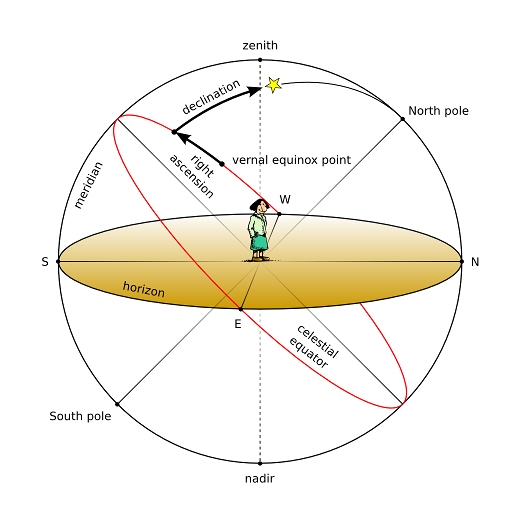
\includegraphics[scale=1.8]{cs_equ}
\caption{Equatorial Coordinates}
\label{fig:EquatorialCoordinates}
\end{figure}

Like the Altitude/Azimuth system, the \indexterm{Right Ascension/Declination}
(RA/Dec) Coordinate System (or \indexterm{Equatorial Coordinate System}) uses two angles to describe positions in the
sky. These angles are measured from standard points on the celestial
sphere. \indexterm{Right ascension} $\alpha$ and \indexterm{declination} $\delta$ are to the celestial sphere what
longitude and latitude are to terrestrial map makers.

The Northern celestial pole has a declination of $\delta=90\degree$, the celestial
equator has a declination of $\delta=0\degree$, and the Southern celestial pole has a declination of $\delta=-90\degree$.

Right ascension is measured as an angle round from a point in the sky
known as the \indexterm{First Point of Aries}, in the same way that longitude
is measured around the Earth from Greenwich. Figure~\ref{fig:EquatorialCoordinates} illustrates
RA/Dec coordinates.

Unlike Altitude/Azimuth coordinates, RA/Dec coordinates of a star do
not change if the observer changes latitude, and do not change over
the course of the day due to the rotation of the Earth (the story is
complicated a little by precession (section~\ref{sec:Concepts:Precession}) and
parallax (section~\ref{sec:Concepts:Parallax}). RA/Dec coordinates are
frequently used in star catalogues such as the Hipparcos catalogue.

Stellarium can draw grid lines for RA/Dec coordinates. Use the button on
the main tool-bar to activate this grid, or press the \key{E} key.

\section{Units}
\label{sec:Concepts:Units}

\subsection{Distance}
\label{sec:Concepts:Distance}

As \name{Douglas Adams} pointed out in the Hitchhiker's Guide to the
Galaxy{[}hhg{]},

\begin{quote}
  Space is big. You just won't believe how vastly, hugely,
  mind-bogglingly big it is. I mean, you may think it's a long way
  down the road to the chemist's, but that's just peanuts to
  space.{[}hhg{]}
\end{quote}
Astronomers use a variety of units for distance that make sense in the
context of the mind-boggling vastness of space.

\begin{description}
\item[Astronomical Unit (AU)] This is the mean Earth-Sun
  distance. Roughly 150 million kilometres
  ($1.49598 \times 10^8\km$). The AU is used mainly when
  discussing the solar system -- for example the distance of various
  planets from the Sun.
\item[Light year (LY)] A light year is not, as some people believe, a
  measure of time. It is the distance that light travels in a
  year. The speed of light being approximately 300,000 kilometres per
  second means a light year is a very large distance indeed, working
  out at about 9.5 trillion kilometres
  ($9.46073\times10^{12}\km$). Light years are most frequently used
  when describing the distance of stars and galaxies or the sizes of
  large-scale objects like galaxies, nebulae etc.
\item[Parsec (pc)] A parsec is defined as the distance of an object
  that has an annual parallax of 1~second of arc. This equates to
  3.26156 light years ($3.08568\times10^{13}\km$). Parsecs (and derivatives: kiloparsec \kpc, megaparsec \Mpc) are most
  frequently used when describing the distance of stars or the sizes
  of large-scale objects like galaxies, nebulae etc.
\end{description}

\subsection{Time}\label{time}

\begin{figure}[h]
\centering\includegraphics[scale=2.2]{sidereal_day}
\caption{Sidereal day}
\label{fig:SiderealDay}
\end{figure}

The length of a day is defined as the amount of time that it takes for
the Sun to travel from the highest point in the sky at mid-day to the
next high-point on the next day. In astronomy this is called a
\emph{solar day}. The apparent motion of the Sun is caused by the
rotation of the Earth. However, in this time, the Earth not only spins,
it also moves slightly round its orbit. Thus in one solar day the Earth
does not spin exactly $360\degree$ on its axis. Another way to measure day
length is to consider how long it takes for the Earth to rotate exactly
$360\degree$. This is known as one \emph{sidereal day}.

Figure~\ref{fig:SiderealDay} illustrates the motion of the Earth as
seen looking down on the Earth orbiting the Sun. The red triangle on the
Earth represents the location of an observer. The figure shows the Earth
at four times:

\begin{enumerate}
\item
  The Sun is directly overhead - it is mid-day.
\item
  Twelve hours have passed since 1. The Earth has rotated round and the
  observer is on the opposite side of the Earth from the Sun. It is
  mid-night. The Earth has also moved round in its orbit a little.
\item
  The Earth has rotated exactly $360\degree$. Exactly one sidereal day has
  passed since 1.
\item
  It is mid-day again -- exactly one solar day since 1. Note that the
  Earth has rotated more than $360\degree$ since 1.
\end{enumerate}

It should be noted that in figure~\ref{fig:SiderealDay} the sizes of
the Sun and Earth and not to scale. More importantly, the distance the
Earth moves around its orbit is much exaggerated. The Earth takes a
year to travel round the Sun --
$365\frac{1}{4}$ solar days. The length of a
sidereal day is about 23 hours, 56 minutes and 4 seconds.

\subsubsection{Sidereal Time}
\label{sec:Concepts:SiderealTime}

It takes exactly one sidereal day for the celestial sphere to make one
revolution in the sky. Astronomers find \indexterm{sidereal time}
useful when observing. This is the Right Ascension which is currently
passing the meridian line.  When visiting observatories, look out for
doctored alarm clocks that have been set to run in sidereal time!



\subsection{Angles}
\label{sec:Concepts:Angles}

Astronomers typically use degrees to measure angles. Since many
observations require very precise measurement, the degree is subdivided
into sixty \emph{minutes of arc} also known as \emph{arc-minutes}. Each
minute of arc is further subdivided into sixty \emph{seconds of arc}, or
\emph{arc-seconds}. Thus one degree is equal to 3600 seconds of arc.
Finer grades of precision are usually expressed using the SI prefixes
with arc-seconds, e.g. \emph{milli arc-seconds} (one milli arc-second is
one thousandth of an arc-second).

\subsubsection{Notation}

Degrees are denoted using the $\degree$ symbol after a number. Minutes of arc are denoted with a~$'$, and seconds of arc are denoted using~$''$. Angles are frequently given in two formats:

\begin{enumerate}
\item
  DMS format --- degrees, minutes and seconds. For example $90\degree15'12''$.
  When more precision is required, the seconds component may include a
  decimal part, for example $90\degree15'12.432''$.
\item
  Decimal degrees, for example $90.2533\degree$
\end{enumerate}

\subsubsection{Handy Angles}
\label{sec:Concepts:Angles:HandyAngles}
\index{Handy Angles}

Being able to estimate angular distance can be very useful when trying
to find objects from star maps in the sky. One way to do this with a
device called a \indexterm{crossbow}.

%% GZ TODO: Add figure of my crossbow!

Crossbows are a nice way get an idea of angular distances, but carrying
one about is a little cumbersome. A more convenient alternative is to
hold up an object such as a pencil at arm's length. If you know the
length of the pencil, $d$, and the distance of it from your eye, $D$, you
can calculate its angular size, $\theta$ using this formula:

\begin{equation}
\label{eq:handyAngle}
\theta=2 \cdot \arctan{\left(\frac{d}{2 \cdot D}\right) }
\end{equation}


\noindent Another, more handy (ahem!) method is to use the size of your hand at
arm's length:

\begin{description}
\item[Tip of little finger] About 1\degree 
\item[Middle three fingers] About 4\degree 
\item[Across the knuckles of the fist] About 10\degree 
\item[Open hand] About 18\degree
\end{description}

Using you hand in this way is not very precise, but it's close enough
to give you some way to translate an idea like ``Mars will be
$45\degree$ above the Southeastern horizon at 21:30''. Of course,
there is variation from person to person, but the variation is
compensated for somewhat by the fact that people with long arms tend
to have larger hands. In exercise~\ref{sec:Exercises:handyAngles} you
will work out your own ``handy angles''.



\subsection{The Magnitude Scale}
\label{sec:Concepts:Magnitudes}


When astronomers talk about magnitude, they are referring to the
brightness of an object. How bright an object appears to be depends on
how much light it is giving out and how far it is from the observer.
Astronomers separate these factors by using two measures: \indexterm{absolute
magnitude} (Mag or $M$) which is a measure of how much light is being
given out by an object, and \indexterm{apparent magnitude} (mag or $m$) which
is how bright something appears to be in the sky.

For example, consider two 100 watt lamps, one which is a few meters
away, and one which is a kilometre away. Both give out the same amount
of light -- they have the same absolute magnitude. However the nearby
lamp seems much brighter -- it has a much greater apparent magnitude.
When astronomers talk about magnitude without specifying whether they
mean apparent or absolute magnitude, they are usually referring to
apparent magnitude.

The magnitude scale has its roots in antiquity. The Greek astronomer
\name{Hipparchus} defined the brightest stars in the sky to be \emph{first
magnitude}, and the dimmest visible to the naked eye to be \emph{sixth
magnitude}. In the 19th century British astronomer \name{Norman Pogson}
quantified the scale more precisely, defining it as a logarithmic scale
where a magnitude~1 object is 100~times as bright as a magnitude~6
object (a difference of five magnitudes). The zero-point of the modern
scale was originally defined as the brightness of the star Vega, however
this was re-defined more formally in 1982\cite{landolt}. Objects brighter
than Vega are given negative magnitudes.

The absolute magnitude of a star is defined as the magnitude a star
would appear if it were 10 parsecs from the observer.

Table~\ref{tab:Concepts:Magnitudes} lists several objects that may be seen
in the sky, their apparent magnitude and their absolute magnitude where
applicable (only stars have an absolute magnitude value. The planets and
the Moon don't give out light like a star does -- they reflect the light
from the Sun).

\begin{table}[htb]
  \centering
%  \begin{tabular}[t]{lll}
%  \end{tabular}
\begin{longtable}[c]{@{}lll@{}}
\toprule
\emph{Object} & $m$ & $M$\tabularnewline
The Sun & -27 & 4.8\tabularnewline
Vega & 0.05 & 0.6\tabularnewline
Betelgeuse & 0.47 & -7.2\tabularnewline
Sirius (the brightest star) & -1.5 & 1.4\tabularnewline
Venus (at brightest) & -4.4 & ---\tabularnewline
Full Moon (at brightest) & -12.6 & ---\tabularnewline
\bottomrule
\end{longtable}
  \caption{Magnitudes of a few objects}
  \label{tab:Concepts:Magnitudes}
\end{table}


\subsection{Luminosity}
\label{sec:Concepts:Luminosity}

\emph{Luminosity} is an expression of the total energy radiated by a
star. It may be measured in watts, however, astronomers tend to use
another expression --- \emph{solar luminosities} where an object with
twice the Sun's luminosity is considered to have two solar luminosities
and so on. Luminosity is related to absolute magnitude.

\section{Precession}
\label{sec:Concepts:Precession}

\begin{figure}[htb]
\centering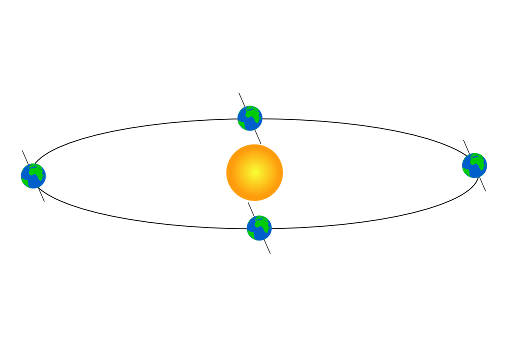
\includegraphics[scale=1.4]{obliquity_ecliptic}
\caption{Ecliptic obliquity}
\label{fig:Obliquity}
\end{figure}

As the Earth orbits the Sun throughout the year, the axis of rotation
(the line running through the rotational poles of the Earth) seems
to point towards the same position on the celestial sphere, as can be
seen in figure~\ref{fig:Obliquity}. The angle between the axis
of rotation and the perpendicular of the orbital plane is called the
\indexterm{obliquity of the ecliptic}. It is currently about $23\degree27'$.

\begin{figure}[htb]
\centering\includegraphics[scale=2.0]{precession}
\caption{Precession}
\label{fig:Precession}
\end{figure}


Observed over very long periods of time the direction the axis of
rotation points to does actually change. The angle between the axis of
rotation and the orbital plane stays fairly constant, but the
direction the axis points --- the position of the celestial pole ---
transcribes a circle on the stars in the celestial sphere. The motion
is similar to the way in which a gyroscope slowly twists, as
figure~\ref{fig:Precession} illustrates. This process is called
\indexterm{precession}. The circles can be shown in Stellarium: From
the View menu (\key{F4}), tab ``Markings'', switch on ``Precession
Circles''.

Precession is a slow process. The axis of rotation twists through a
full $360\degree$ about once every 28,000 years. However, over these
long times other gravitational perturbations (``planetary
precession'') play a role, and what may be thought of as rigid
``precession circle'' can actually only show the instantaneous
(current) state. Over millennia the circle slightly varies.

Precession has some important implications:

\begin{enumerate}
\item RA/Dec coordinates change over time, albeit slowly. Measurements
  of the positions of stars recorded using RA/Dec coordinates must
  also include a date (``equinox'') for those coordinates. Therefore
  the current star catalogues list their objects for the epoch and
  equinox J2000.0.
\item
  Polaris, the pole star, won't stay a good indicator of the location of
  the Northern celestial pole. In 14,000 years time Polaris will be
  nearly $47\degree$ away from the celestial pole!
\end{enumerate}


\section{Parallax}
\label{sec:Concepts:Parallax}


Parallax is the change of angular position of two stationary points
relative to each other as seen by an observer, due to the motion of said
observer. Or more simply put, it is the apparent shift of an object
against a background due to a change in observer position.

This can be demonstrated by holding ones thumb up at arm's length.
Closing one eye, note the position of the thumb against the background.
After swapping which eye is open (without moving), the thumb appears to
be in a different position against the background.

\subsection{Geocentric and Topocentric Observations}
\label{sec:Concepts:Topocentric}

%% Author GZ 2016-01-11

When computing planetary positions was done manually by adding numbers
tabulated in yearly almanacs, computing the Earth's position and, say,
position of a minor planet was usually good enough to find the object
in the sky. In both cases, the exact numbers refer to the
gravitational centres of the respective bodies. However, we are
sitting on Earth's surface, so the observed planet will be seen in a
slightly shifted location. The amount for objects in the inner solar
system is usually just a few arcseconds and indeed negligible when we
just want to find an object. But it makes a difference when it comes
to observations of stellar occultations by planets or asteroids. Such
a body may measure only a few tens of kilometres, so the shadow track
which it leaves on Earth's surface is of approximately the same
size.\footnote{Unfortunately Stellarium (as of V0.14) is not accurate
  enough to reliably compute such occultations. Even a deviation of
  0.5 arcseconds is too much here.}

A much closer and bigger object is the Moon, which can also occult
stars. It can even occult the one big star we call the Sun: this is a
Solar Eclipse. And here it makes a huge difference where on the planet
you are located. 

If you are interested in astronomical computing, you may still be
interested in geocentric numerical results. From the Settings panel
(\key{F2}), tab ``Tools'', there is a checkbox for ``Topocentric
Coordinates''. Switch it off to put yourself into the center of the
planet you are located.

\subsection{Stellar Parallax}
\label{sec:Concepts:StellarParallax}

\begin{figure}[tb]
\centering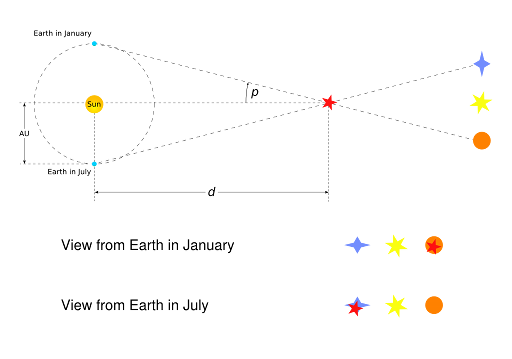
\includegraphics[scale=2.0]{parallax}
\caption{Stellar Parallax}
\label{fig:Parallax}
\end{figure}

A similar thing happens due to the Earth's motion around the Sun. Nearby
stars appear to move against more distant background stars, as
illustrated in figure~\ref{fig:Parallax}.
The movement of nearby stars against the background is called
\emph{stellar parallax}, or \emph{annual parallax}.

Since we know the distance the radius of the Earth's orbit around the
Sun from other methods, we can use simple geometry to calculate the
distance of the nearby star if we measure annual parallax.

As can be seen from figure~\ref{fig:Parallax}, the annual
parallax $p$ is half the angular distance between the apparent positions
of the nearby star. The distance of the nearby object is $d$. Astronomers
use a unit of distance called the parsec ($\pc$) which is defined as the
distance at which a nearby star has $p=1''$.

Even the nearest stars exhibit very small movement due to
parallax. The closest star to the Earth other than the Sun is Proxima
Centauri. It has an annual parallax of $0.77199''$, corresponding to a
distance of $1.295\pc$ (4.22 light years).

Even with the most sensitive instruments for measuring the positions of
the stars it is only possible to use parallax to determine the distance
of stars up to about 1,600 light years from the Earth, after which the
annual parallax is so small it cannot be measured accurately enough.

In Stellarium, the annual parallax can be listed in the object information for stars
when available. It is not used for the positional calculations.

\section{Proper Motion}
\label{sec:Concepts:ProperMotion}

\indexterm{Proper motion} is the change in the position of a star over time as a
result of its motion through space relative to the Sun. It does not
include the apparent shift in position of star due to annular parallax.
The star exhibiting the greatest proper motion is \indexterm{Barnard's Star} which
moves more than ten seconds of arc per year.

If you want to simulate the effect of proper motion with Stellarium,
put the map into equatorial view mode, switch off ground and cardinal
marks, and set some high time lapse speed. You will see a few stars
change their locations quite soon, those are usually stars in our
galactic neighbourhood.

Note however some limitations:
\begin{enumerate}
\item Stellarium will stop at $\pm 100.000$ years. This limit may be
  still suitable for the stellar locations. The planetary locations
  are not trustworthy outside of a much closer temporal window (see
  section~\ref{sec:Accuracy}). You cannot simulate the sky over the
  dinosaurs or such things.
\item Proper motion is only modelled by the linear components. True 3D
  motion in space requires more computation, which would slow down the
  program.
\item Double stars are listed in catalogs as two individual stars with
  their current proper motion. They may be seen flying apart, which is
  of course not realistic.
\end{enumerate}

%%% Local Variables: 
%%% mode: latex
%%% TeX-PDF-mode: t
%%% TeX-master: "guide"
%%% End: 
